\documentclass{beamer}

\usepackage{beamerthemesplit}

\usetheme{Pittsburgh}
\usecolortheme{seagull}

\usefonttheme{serif}

\newcommand{\snT}{$(S/N)_{size}$}
\newcommand{\snflux}{$(S/N)_{flux}$}

\title{Shear Estimation}
\author
{
    Erin Sheldon \\
    Brookhaven National Lab
}

\begin{document}

\frame{\titlepage}

\section{Introduction}

\frame
{
    \frametitle{Abell 370, HST}
    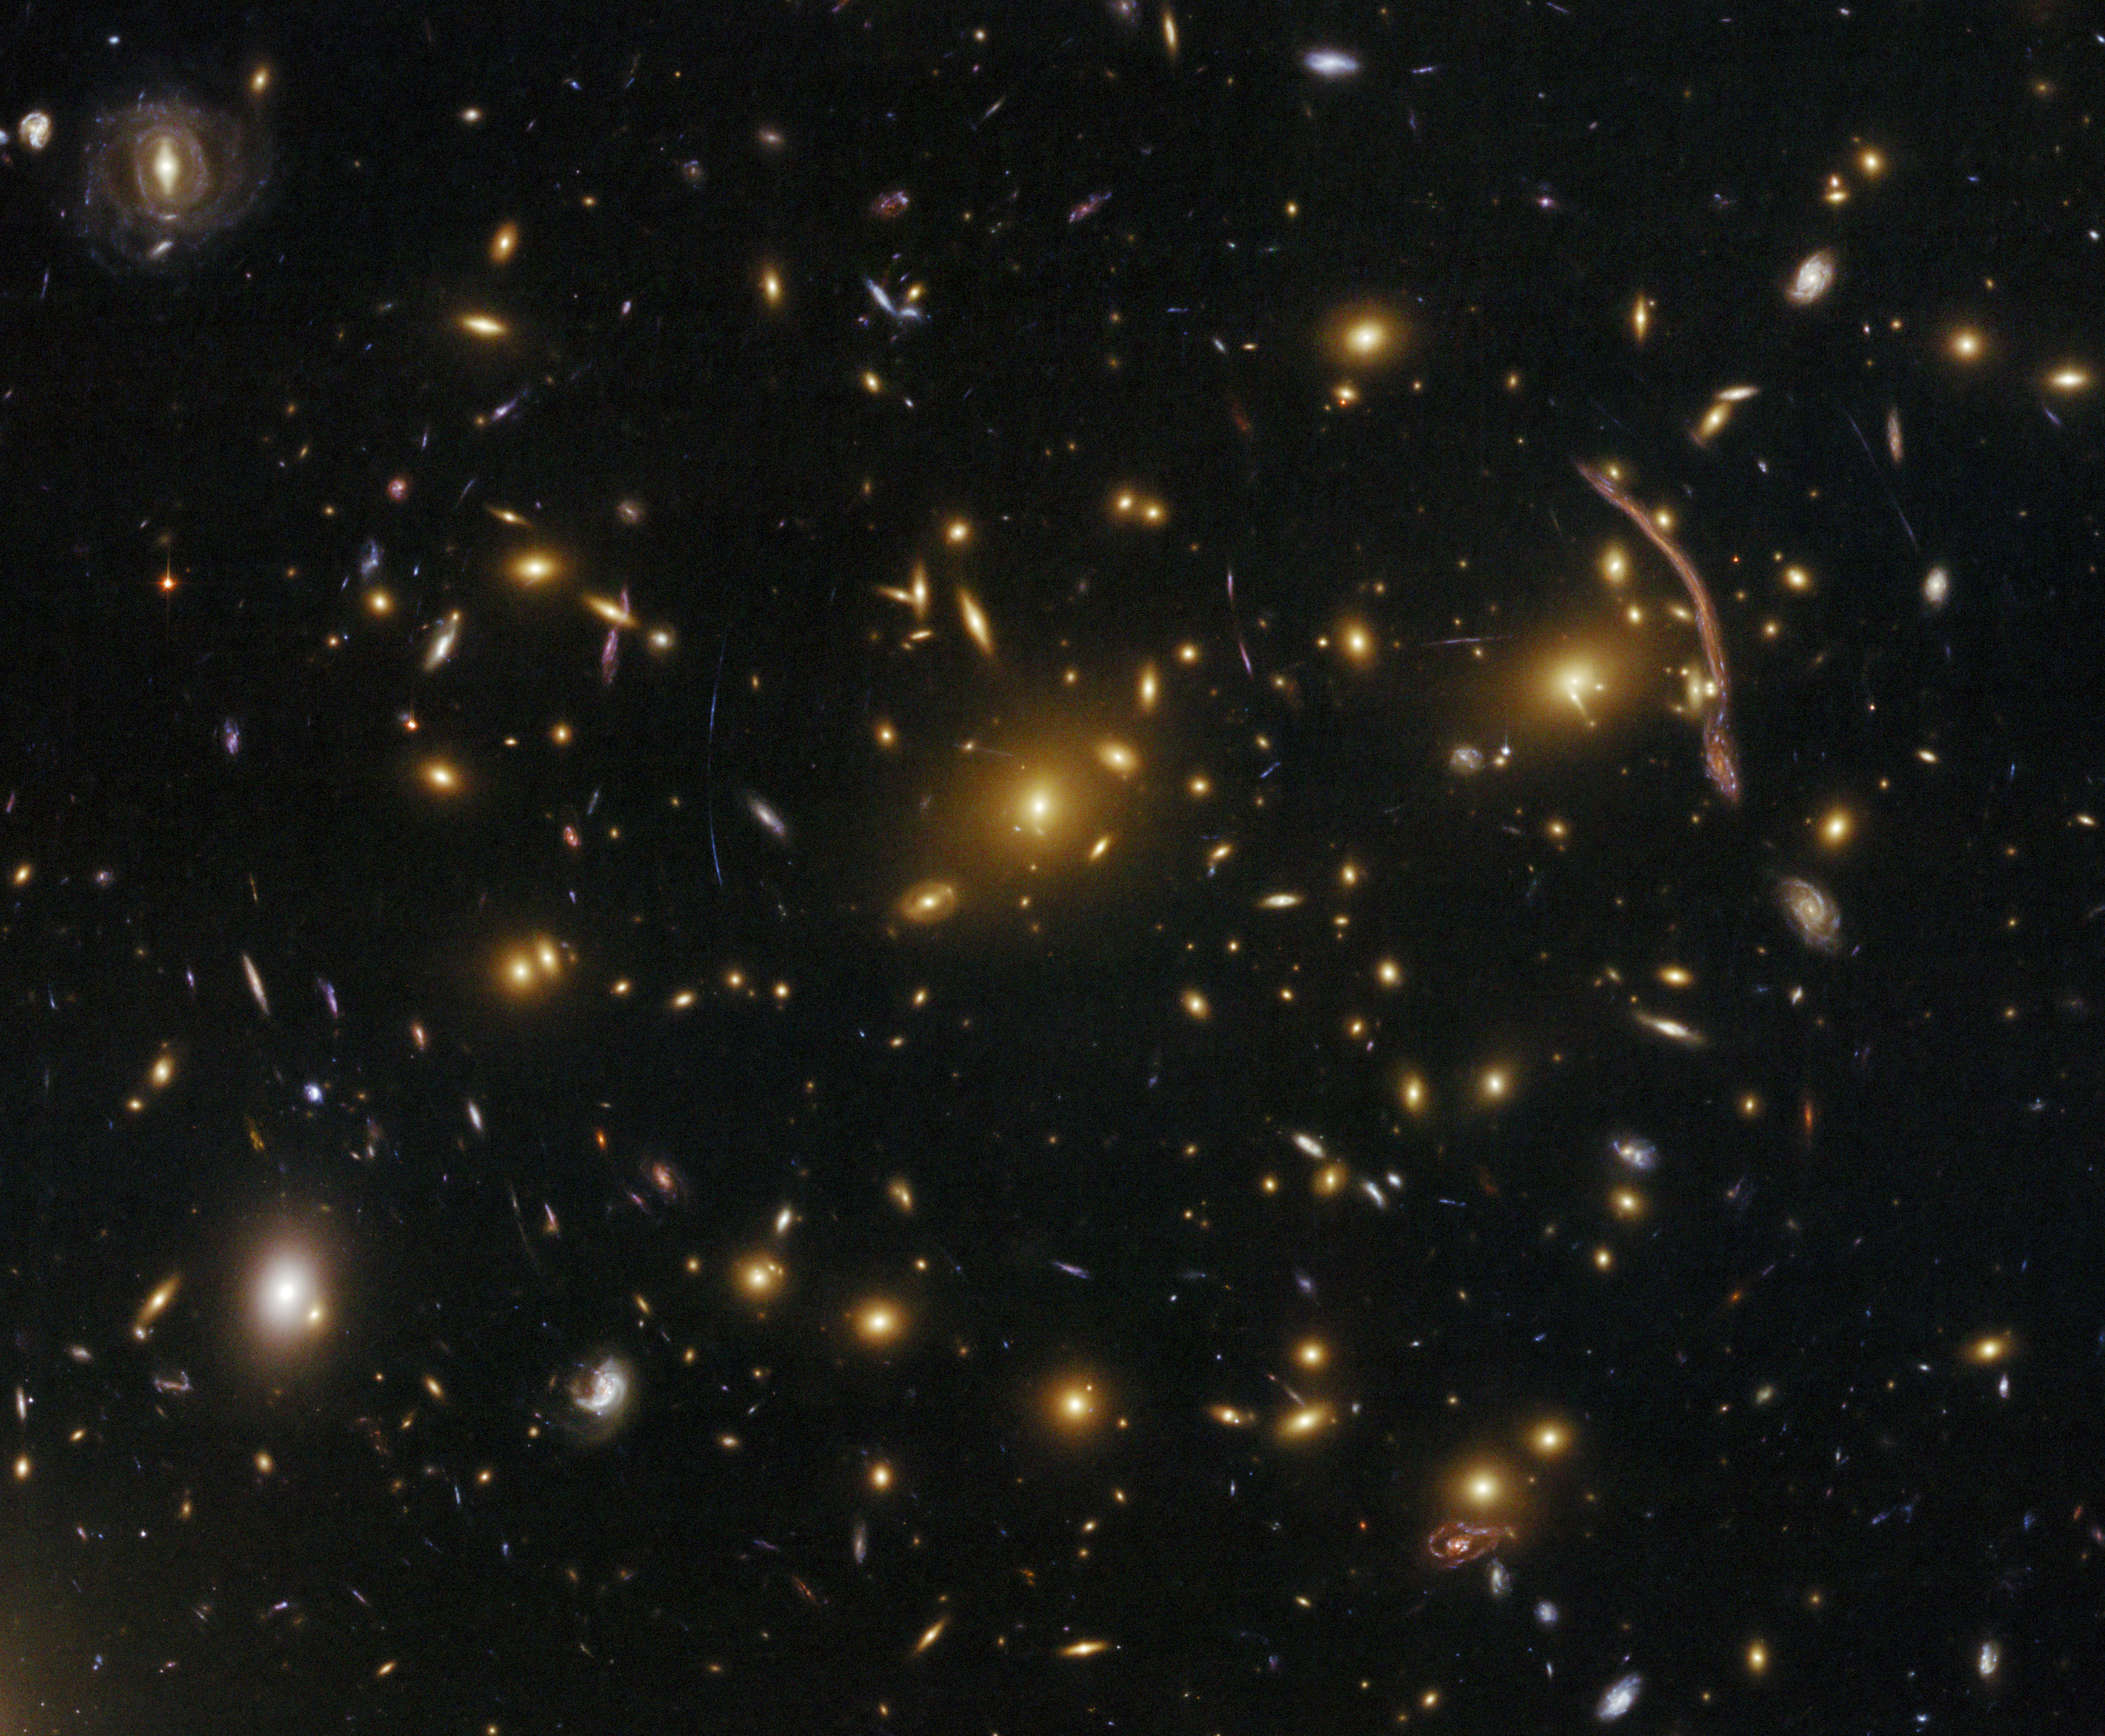
\includegraphics[width=\textwidth]{abell370_hst_med.jpg}
}
\frame
{
    \frametitle{Lensing Geometry and Deflection}
    \includegraphics[width=\textwidth]{lens_geometry.pdf}
}

\frame
{
    \frametitle{Shear Illustration}
    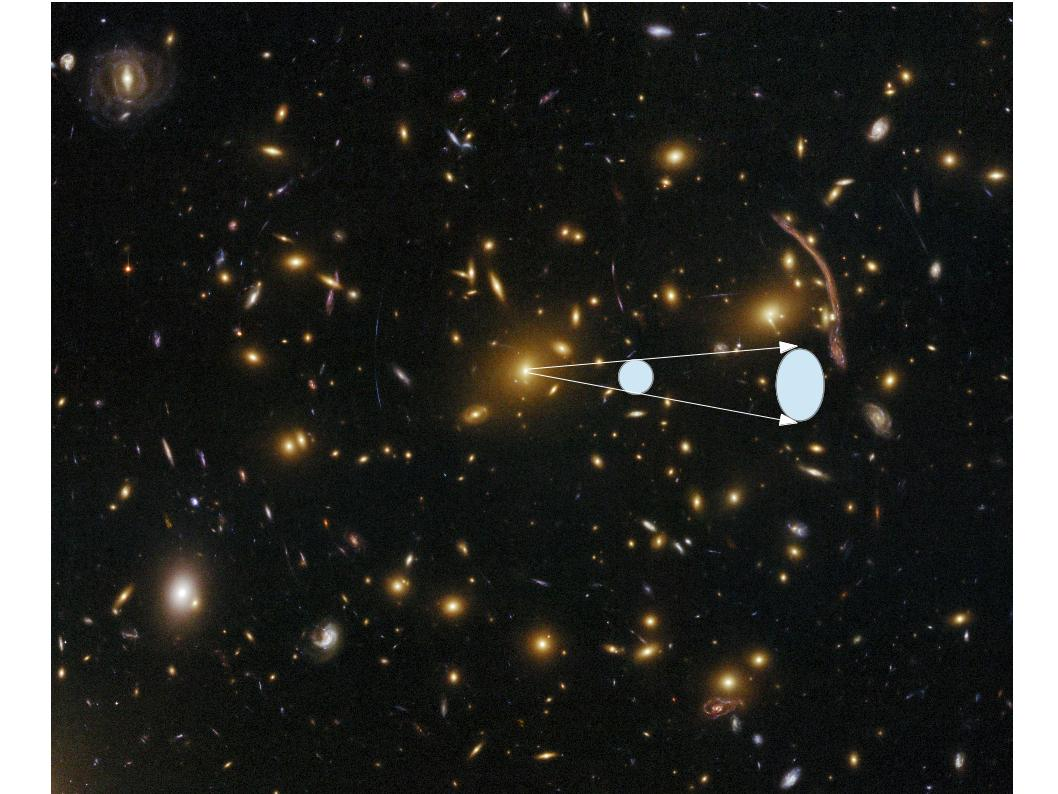
\includegraphics[width=\textwidth]{shear-illustration.jpg}
}



\frame
{
    \fontsize{10}{\baselineskip}

    \frametitle{Gravitational Shear}

    \begin{columns}

        \begin{column}{0.5\textwidth}

            \begin{itemize}
                \item The path of light appears curved as it passes massive objects
                \item The ``deflection'' can differ across the face of an extended source galaxy, causing distortion.
                \item Shear distorts the image; we say it's ``shape'' is altered.
                \item Shearing produces correlations in the shapes of galaxies across the sky.
                    Shape correlations are closely related to mass density
                    correlations.

            \end{itemize}
        \end{column}
        \begin{column}{0.5\textwidth}
            \includegraphics[width=\textwidth]{shear-illustration-crop.jpg}
            \newline
            Note galaxies aren't round!  ``Shape noise''
        \end{column}
    \end{columns}
}



\frame
{
    \frametitle{Measuring Shear}

    \begin{itemize}
        \item For a perfect detector with no noise, just measure
            the second moments and look for the correlations.
        \item The atmosphere, telescope, and instrument smear
            the image: the Point Spread Function (PSF).
        \item That just adds to the moments, so we just need to
            subtract off the PSF moments!
        \item .... but there is noise, so the moments don't converge (among
            other difficulties).
    \end{itemize}
}

\frame
{
    \frametitle{PSF and Noise}
    
    \begin{itemize}

        \item One can use a weight function to suppress the noise, but then one
            must derive how that measurement responds to smearing by the PSF
            and shearing (e.g. Kaiser, Squires, \& Broadhurst, Bernstein \& Jarvis, Melchior,
                    Bernstein \& Armstrong).  Working in Fourier space can help
            with the deconvolution (Bernstein).

        \item Alternatively, one can forward-model the problem: fit a model that is
            convolved with an estimate of the PSF.  Limited by how well one can
            model the galaxy and PSF (e.g. Miller et al., Bernstein \& Armstrong, many
            others).

        \item These methods can be made to work pretty well, as long as
            the $S/N$ is still pretty high, say 50 or higher.

    \end{itemize}
}

\frame
{
    \frametitle{Noise}

    \begin{itemize}
        \item When the $S/N$ is low, these techniques break down.
        \item Non-linear fitting in the presence of noise is biased, both
            the maximum likelihood and expectation value: using the mean
            shape won't work (Hirata, Refregier, etc).  This is well 
            known in statistics. Badly aggravated by the PSF ``deconvolution''.
        \item The noise also causes problems for moment based methods.
    \end{itemize}
}

\frame
{
    \frametitle{Miller et al. 2007}

    \begin{itemize}

        \item Miller et al. 2007 (LENSFIT): Use priors on the parameters and
            explore full posterior surface (Prior $\times$ Likelihood).
            Attempt to derive how the shear estimate (the shape) is affected by
            the noise and prior using integrals over the posterior surface and
            first order approximation in shear.

        \item The posterior surface of the shape for a single galaxy is
            complex.  The space is bounded, the surface is necessarily
            asymmetric and depends on galaxy properties and noise. No generic
            formulation can be made for the response, rather an ad-hoc method
            is used.  Miller et al. 2013 find large biases in simulations, of
            order 10\%.
        
    \end{itemize}
}

\frame
{
    \frametitle{LENSFIT Tests}

    \begin{columns}
        
        \begin{column}{0.5\textwidth}
            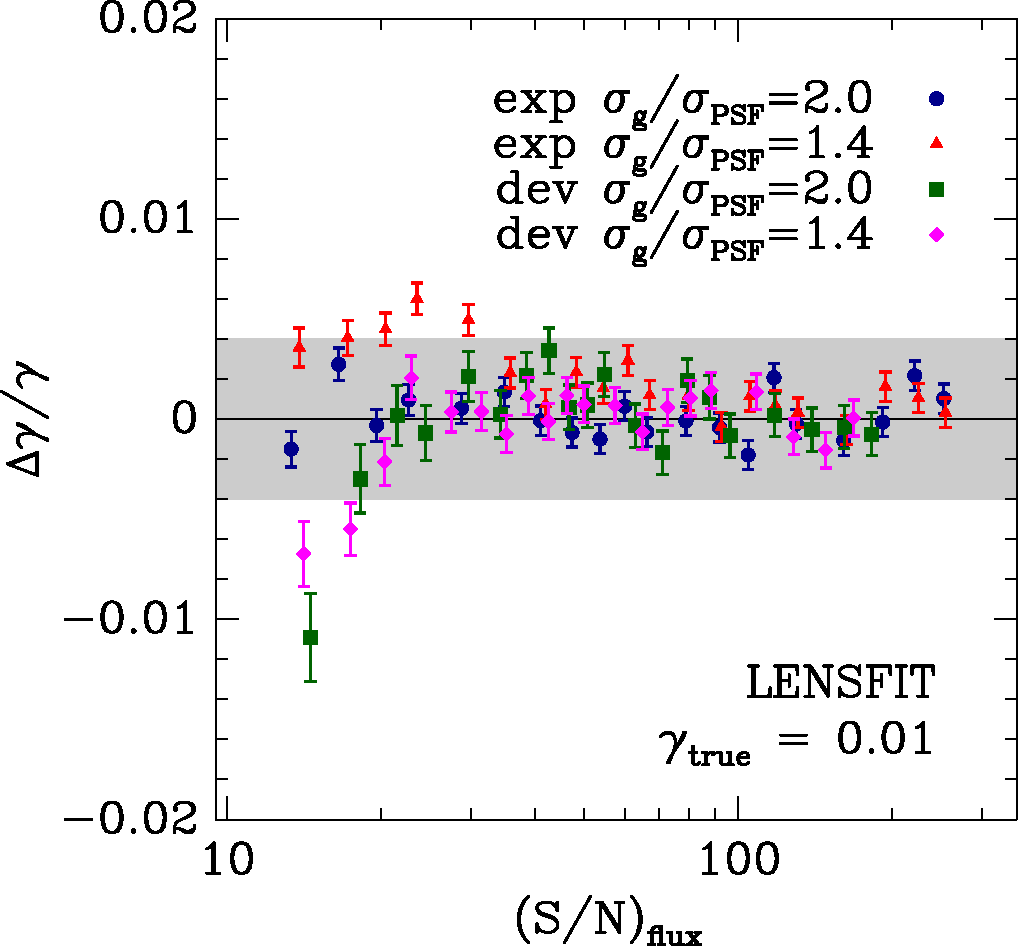
\includegraphics[width=\textwidth]{cbafit-geg07-geg08-deg03-deg05-lensfit-flux-s2n.pdf}
        \end{column}

        \begin{column}{0.5\textwidth}
            \includegraphics[width=\textwidth]{cbafit-geg07-geg08-deg03-deg05-lensfit-T-s2n.pdf}
        \end{column}
    \end{columns}

    \begin{itemize}
        \item I did my own tests of LENSFIT with strong structural priors (15\% wide).

        \item Very fast code using gaussian mixtures to approximate galaxies.  Fast
            analytic convolutions.

        \item Bias vs \snT\ has more universal form than vs \snflux.
    \end{itemize}

}

\frame
{
    \frametitle{Shear of the Light Distribution}

    \begin{itemize}

        \item Stack the light around peaks in images.

        \item Assume the shear is constant over the patch of interest.

        \item This two-dimensioinal correlation function of the light is
            sheared just as galaxy images are.  Don't need to de-blend.  Not
            fully explored (ES).

    \end{itemize}
}
\frame
{
    \frametitle{Bernstein \& Armstrong 2013}

    \begin{itemize}

        \item Shape is not shear.
        \item While the posterior surface for the {\it shape} of single galaxy
            is complex, the posterior surface for the {\it mean shear} of an
            ensemble must approach a Gaussian according to the central limit
            theorem.  This is actually true!

         \item With the Gaussian assumption, and assumption of weak
             shear, can derive an unbiased estimator for the mean shear.

         \item You lose nothing: in the limit of weak shear, you need
             to use an ensemble statistic anyway.  The ``shape noise'',
             intrinsic variance in shapes of galaxies, dominates over
             the signal. XXX introduce shape noise earlier.

        \item This is a good idea, but needed an implementation, so I worked it
            into my existing code.
         
    \end{itemize}

}

\frame
{
    \frametitle{BA13 Tests}

    \begin{columns}
        
        \begin{column}{0.5\textwidth}
            \includegraphics[width=\textwidth]{cbafit-geg07-geg08-deg03-deg05-pqr-flux-s2n.pdf}
        \end{column}

        \begin{column}{0.5\textwidth}
            \includegraphics[width=\textwidth]{cbafit-geg07-geg08-deg03-deg05-pqr-T-s2n.pdf}
        \end{column}
    \end{columns}
}

\frame
{
    
    \frametitle{Bernstein \& Armstrong 2013 Tests}

    \begin{itemize}
        \item Can push to lower \snT\ than LENSFIT.
        \item Bias varies with \snT\ in a simpler way than LENSFIT.
        \item Bias vs \snT\ even more universal.
        \item TODO: explore more realistic intrinsic distributions in structural
            parameters (size, flux).  E.g. for a bin in measured flux, what are
            the {\it true} distributions in size and flux?  Use Cosmos.
    \end{itemize}
}

\end{document}
